\documentclass[envcountsame]{llncs}
%\usepackage[margin=1in]{geometry} 
%\usepackage{amsmath,amsthm,amssymb,scrextend}
\usepackage{amsmath}
\usepackage{fancyhdr}
\usepackage{bbold}
\pagestyle{fancy}
\usepackage{natbib}
\usepackage[noend]{algpseudocode}
\usepackage{algorithm}
\usepackage{nomencl}
\usepackage{bm}
\usepackage{tikz}
\usepackage{tikz-cd}
\usepackage{graphicx}
\usetikzlibrary{arrows}
\usetikzlibrary{matrix,arrows,decorations.pathmorphing}
\usepackage{scalefnt}
\usepackage{tikz-qtree}
\usepackage{subfigure} 

\usetikzlibrary{shapes,positioning,chains,fit,calc}
\usetikzlibrary{decorations.markings}
\tikzstyle arrowstyle=[scale=1]
\tikzstyle directed=[postaction={decorate,decoration={markings,
		mark=at position .65 with {\arrow[arrowstyle]{stealth}}}}]
\tikzstyle reverse directed=[postaction={decorate,decoration={markings,
		mark=at position .65 with {\arrowreversed[arrowstyle]{stealth};}}}]

\usepackage{caption} 
\captionsetup[table]{skip=10pt}
\makenomenclature
\renewcommand{\nomname}{List of Symbols}
 
\renewcommand{\nompreamble}{The next list describes several symbols that will be later used within the body of the document}

\begin{document}
	
	% --------------------------------------------------------------
	%                         Start here
	% --------------------------------------------------------------
	
	%\lhead{Centrality}
	%\chead{Sketch work}
	%\rhead{\today}
	\title{1. Centrality with Commodity Loss\\
    2. Group Centrality for Flow Networks\\
    3. Centrality Measures in an Electric Vehicle Wireless Charging Lane Road Network}
	\author{Hayato Ushijima-Mwesigwa \and Ilya Safro}
	\institute{School of Computing, Clemson Univesity, Clemson, SC 29634\\
	\email{(hushiji, isafro)@clemson.edu}	
}

	\maketitle
	\begin{abstract}
This paper extends the betweenness, eigenvector, and degree-like centrality measures for applications that have a component of commodity loss.  This work is motivated by the concept of an Electric Vehicle (EV) traveling on a road network equipped with in-motion wireless charging lanes. Each EV on the network has an on-board battery with limited charge. Thus, it is not guaranteed that EV can arrive from one destination to another even if the network is connected. On question of interest is,``what are the important lanes in the network?''. In water networks, pressure gradients act as the driving force of water from source to demand.  An optimal pump scheduling problem is one that provides an operator with the least-cost operation policy for all pump stations in the network in order to satisfy the demand at a given time.  In this work, the authors consider a \emph{walker} in a network, where the walker has limited energy, thus limited range. Centralities based on the type of walk the walker takes are discussed. 

This work studies the importance on nodes in EV-wireless charing road networks. 
	\end{abstract}
	
	\noindent\textbf{Keywords:} Centrality,
	\section{Introduction}
 
 How does the deployment of wireless charing lanes in a road network affect the importance of a node in the network? What are the central nodes in the network with respect to a given deployment?
 
What does it mean to be an \emph{important} node in a EV-road network with wireless charging lanes. The following summarize a few scenarios
\begin{enumerate}
\item Node $v$ is important if it is a good starting location for a EV in the network. \emph{What does a good starting location mean?} Assume that an EV starts fully charged, a good starting location could mean:
\begin{enumerate}
\item Has the ability to arrive at large number of nodes in the network
\item Has the ability to complete a large percentage of any route it takes.
\end{enumerate}
These can been viewed as \emph{radial measures}
\item A node is a good installation location. This importance is based on whether or not other nodes have WCL installed on them. This can be viewed as a \emph{medial measure}
\end{enumerate}
\nomenclature{$\delta_{s,t}^i$}{Number of shortest $s$-$t$ feasible paths of length $i$}%
\nomenclature{$\delta_{s,t}^i(v)$}{Number of shortest $s$-$t$ feasible paths of length $i$, that pass through node $v$}%
\nomenclature{$\alpha_i$}{Parameter giving more importance to paths of shorter length}%
%\nomenclature{$P_{s,t}^i$}{The set of shortest paths from $s$ to $t$ of 
\printnomenclature


\subsection{Applications}

\cite{sarkar2011random} Real world applications such as friend suggestion in social networks, keyword search in databases, web-spam detection etc. can be framed as ranking entities of a graph. Ranking using random walks is an active area of research. 

Problems that can be framed as ranking problems in graph include
\begin{enumerate}
\item Suggesting friends to a new user in an online social network
\item Movie and music recommendation
\item Keyword search in large publication databases. Find papers which are "contextually" similar to the query submitted by the user. 

\end{enumerate}
Work related to random walks
\begin{enumerate}
\item Clustering
\item Semi-supervised learning
\item 
\end{enumerate}


	\section{Radial Measures}
     With regard to the current state of the road network (WCL deployment), how important is a given node as a potential starting location? If all vehicles in the network have range of the entire network, then this would be equal to the standard betweenness centrality, that is, only topological importance is considered. An important node is one that adds more range to the entire network. 
%	Redial measures are one where a walk originates from a node.  The two most common radial measures are 
%	\subsection{Degree-like centrality}
%	Degree centrality counts the number of walks of length one that originate from a node. 
%	\subsection{Closeness-like centrality}
%	\emph{Closeness centrality} is defined as the total geodesic distance from a given node to all other nodes. Since the number of nodes is fixed in a network, this measure is equivalent to the mean distance of a node to all other nodes. In terms of a WCL installation, each EV has a limited range within the network. For a given network, define the \emph{energy deficiency} between two nodes $u,v$ as the  additional energy a walker needs to arrive a node $v$ from $u$. Note that this can vary depending on the type of walk the walker is taking.  

\subsection{Eigenvector Centrality}
Eigenvector centrality is based on random walks. 

Let $G=(V,E)$ be a graph with adjacency matrix $A$ and $|V|=n$. For any set $V' \subset V$, define the diagonal matrix $I_X$ as
\begin{equation*}
(J(V'))_{ii}= (J)_{ii} = \begin{cases}
1, & \text{if } i \in V' \\
0, & \text{otherwise} 
\end{cases}
\end{equation*}
Let $I$ be the $n\times n$ identity matrix and, for some fixed value $k \in \mathbb{N}$, define the $nk \times nk$  block matrix $\mathcal{B}_k$ as 


\begin{equation*}
\mathcal{B}_k = \begin{pmatrix}
 AJ & A(I-J) & 0& \dots& \dots& \dots& 0\\\
AJ & 0 & A(I-J) &0& \dots& \dots &0 \\
 AJ & 0 &0 & \ddots &0& \dots &0 \\
\vdots & & & & \ddots & & \vdots\\
\vdots & & & &  & \ddots & \vdots\\
AJ& 0 &0 & \dots &0& \dots A(I-J)\\
 AJ& 0 &0 & \dots &0& \dots &0\\
\end{pmatrix}
\end{equation*}
We are interested in determining the spectral properties of $\mathcal{B}_k$ in terms of $A$?

Consider the case when $k=2$, then we have the $\mathcal{B}_2$ as
\begin{equation*}
\mathcal{B}_2 = \begin{pmatrix}
A J & A(I-J)\\\
 AJ & 0 \\
\end{pmatrix}
\end{equation*}
%The eigenvalues of $\mathcal{B}_2$ are given by $\lambda$ such that the determinant of 
%\begin{equation*}
% \begin{pmatrix}
%J A - \lambda I& (I-J)A\\\
%J A & - \lambda I \\
%\end{pmatrix}
%\end{equation*}
%is zeros. Since $JA$ and $\lambda I$ commute we have the equation
%\begin{align*}
%0=&\det ((JA- \lambda I)(-\lambda I) - (I-J)AJA) \\
%= & \det (\lambda (JA- \lambda I) + (I-J)AJA) \\
%\end{align*}

\subsection{Counting Number of Feasible Walks}
The $i$-$j$th entry of the matrix $A^k$ for some $k$ counts from $i$ to $j$ of length $k$. However, not all of these walks are in fact feasible. This leads to the interesting question of finding a matrix that represents the number of $i$-$j$ feasible walks. Here a feasible path is defined as one that starts with full charge/energy.

Consider the matrix $\mathcal{B}_m^k$. Assume that the index of nodes in $V$ and matrices $I,J,A, \mathcal{B}_m$ start at 0. For $0 \leq i < n$, $0 \leq i' < nk$,  and $j \equiv \pmod{n}$, the $i$-$j$th entry of $\mathcal{B}_m^k$ gives the number of walks from node $i$ to $j$  completing with a the different charges where $i,j\in V$. The destination charge is given by the value $\lfloor i'/n \rfloor$. This implies that the number of walks from $i$ to $j$ ending with non-negative charge is given by the summation at each discrete charge level. 

Let $\mathcal{I}_k$ be an $nm \times n$ block matrix with $m$ blocks of identity matrix $i$ given by
\begin{equation*}
\mathcal{I}_m
\begin{bmatrix}
I \\
I \\
\vdots \\
I
\end{bmatrix}, \quad
\mathcal{Z}_m
\begin{bmatrix}
I \\
0 \\
\vdots \\
0
\end{bmatrix}
\end{equation*}

We claim that the matrix  $\mathcal{I}_m^T\mathcal{B}_m^k\mathcal{I}_m$, is an $n\times n$ matrix whose $i$-$j$th entries give the number of feasible walks from $i$ to $j$ of length $k$. 

Let $S$ be the $nm \times nm$ matrix with $i$-$j$ term given by
\begin{equation*}
s_{ij} = \sum_{k=1}^{\infty}\alpha^k[\mathcal{B}_m^k]_{ij}
\end{equation*}
Thus,
\begin{align*}
S &= I_{nm \times nm} + \alpha \mathcal{B}_m + \alpha^2 \mathcal{B}_m^2 + \dots +  \alpha^i \mathcal{B}_m^i + \dots \\
&= (I_{nm \times nm} - \alpha \mathcal{B}_m )^{-1}
\end{align*}
Then, if $W$ is the $n \times n$ matrix given
\begin{equation*}
W =  \mathcal{Z}_m^T(I_{nm \times nm} - \alpha \mathcal{B}_m )^{-1}\mathcal{I}_m
\end{equation*}
The centrality is then given by $C = W \textbf{1}$.

For a standard graph, the Katz centrality is computed by $(I - \alpha A)^{-1}$. The parameter $\alpha$, also known as the \emph{damping factor} must be chosen carefully such that $0 < \alpha < 1/\lambda_{\max}$. If $\alpha \to 0$, then only walks of very short length are taken into account. 

\begin{theorem}
$\lambda_{max}(A) > \lambda_{max}({\mathcal{B}})$ .
\label{lamda}
\end{theorem}
\begin{proof}
If $\mathcal{A} = \mathcal{Z}_m^T\mathcal{B}_m \mathcal{I}_m$, then $\mathcal{A}^k$ is the $n \times n$ matrix that counts the walks of length $k$ in the bounded-walk graph. Clearly, $[A^k]_{ij} \geq [\mathcal{A}^k]_{ij}$ for all $i,j$. This implies that if the sequence $\{\alpha^k A^k\}_{k=1}^{\infty}$ converges, then $\{\alpha^k \mathcal{A}^k\}_{k=1}^{\infty}$ converges. Thus, $\lambda_{max}(A) > \lambda_{max}({\mathcal{B}})$ 
\end{proof}
Theorem \ref{lamda} is useful in that walks of longer length are taken into account. A good placement is one that maximizes $ \lambda_{\max}({\mathcal{B}})$

\begin{figure}[ht]
	\begin{center}
		\begin{tikzpicture} [scale = 1]
     \draw (0,0) -> (1.2, 1);
     \draw (0.5,0) -> (1.2, 1);
     \draw (1,0) -> (1.2, 1);
     \draw (1.5,0) -> (1.2, 1);
     \draw (2,0) -> (1.2, 1);
     \draw (2.5,0) -> (1.2, 1);
     \draw (1.2,1) -> (2,2);
     
     \draw (5,0) -> (6.2, 1);
     \draw (5.5,0) -> (6.2, 1);
     \draw (6,0) -> (6.2, 1);
     \draw (6.5,0) -> (6.2, 1);
     \draw (7,0) -> (6.2, 1);
     \draw (7.5,0) -> (6.2, 1);
     \draw (6.2,1) -> (5.5,2);
     \draw (5.5,2) -> (2,2);
     \draw [fill=white] (2,2) circle [radius=0.1] node[above]{$u_3$};
     \draw [fill] (0,0) circle [radius=0.1]node[left]{$u_1$};
     \draw [fill] (0.5,0) circle [radius=0.1];
     \draw [fill] (1,0) circle [radius=0.1];
     \draw [fill] (1.5,0) circle [radius=0.1];
     \draw [fill] (2,0) circle [radius=0.1];
     \draw [fill] (2.5,0) circle [radius=0.1];
     \draw [fill] (1.2,1) circle [radius=0.1] node[left]{$u_2$};
     \draw [fill] (5,0) circle [radius=0.1];
     \draw [fill] (5.5,0) circle [radius=0.1];
     \draw [fill] (6,0) circle [radius=0.1];
     \draw [fill] (6.5,0) circle [radius=0.1];
     \draw [fill] (7,0) circle [radius=0.1];
     \draw [fill] (7.5,0) circle [radius=0.1]node[right]{$u_6$};
     \draw [fill] (5.5,2) circle [radius=0.1]node[above]{$u_4$};
     \draw [fill] (6.2,1) circle [radius=0.1]node[right]{$u_5$};
		\end{tikzpicture}
	\label{fig:twopath}
	\end{center}
    \caption{Example to demonstrate different centrality measures}
\end{figure}


\begin{table}
\centering
\begin{tabular}{ lccc}
\hline
Node~ & ~Katz~ & ~Katz2 ~ & Bounded-Katz \\ \hline
  $u_1$ & 0.19 &0.19  &0.16\\ \hline
 $u_2$ &0.48  &0.48   &0.76\\ \hline
$\bm{u_3}$& 0.30 & \textbf{0.31} &0.31\\ \hline 
$\bm{u_4}$ &0.30 &0.30   &\textbf{0.33}\\ \hline 
$u_5$ & 0.48 &  0.47&0.17\\ \hline 
$u_6$ & 0.19 & 0.19&0.11\\ \hline 
\end{tabular}
\caption{Normalized centrality values: If $u_3$ is a verified user, it doesn't particular help it to spread information, however, it should help $u_4$ thus $u_4$ should be more influential than $u_3$}
\end{table}



\begin{figure}[t]
\centering
\subfigure[$\Gamma =2$]{
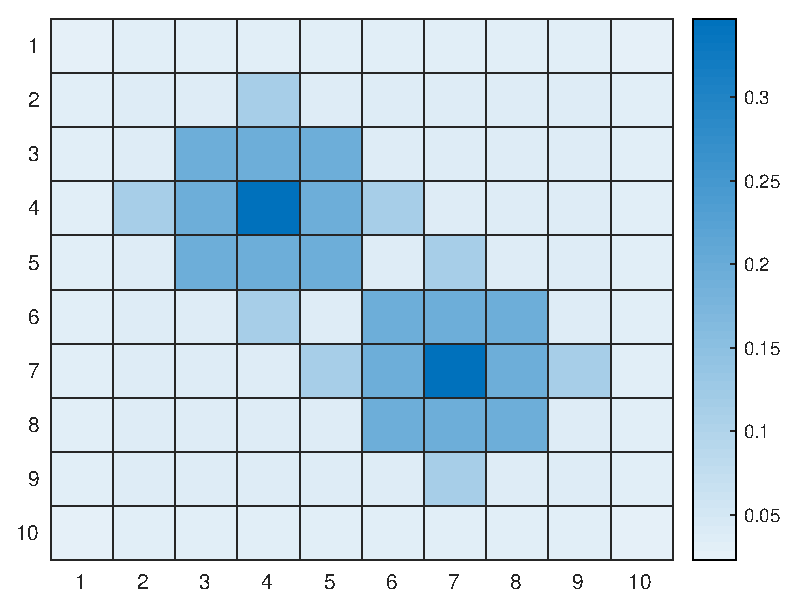
\includegraphics[width=.3\textwidth]{./fig/grid2}
}
\subfigure[$\Gamma =4$]{
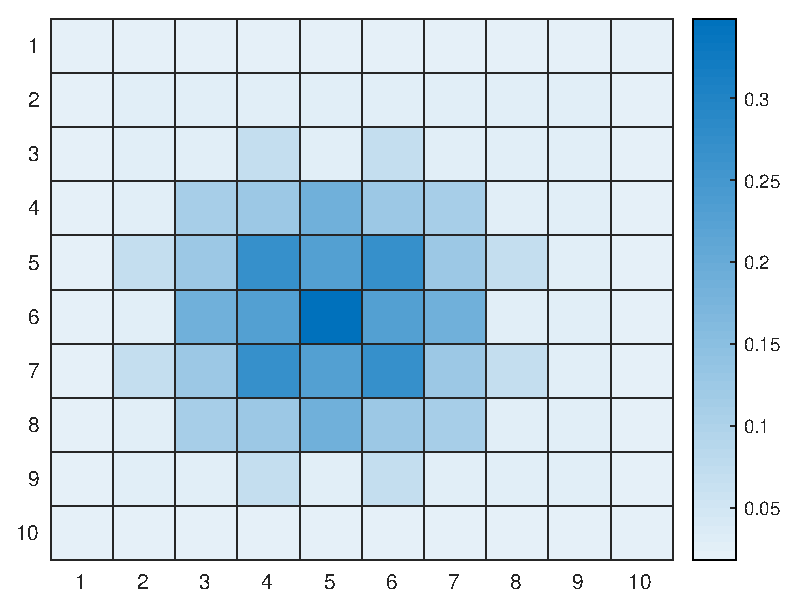
\includegraphics[width=.3\textwidth]{./fig/grid4}
}
\subfigure[$\Gamma =10$]{
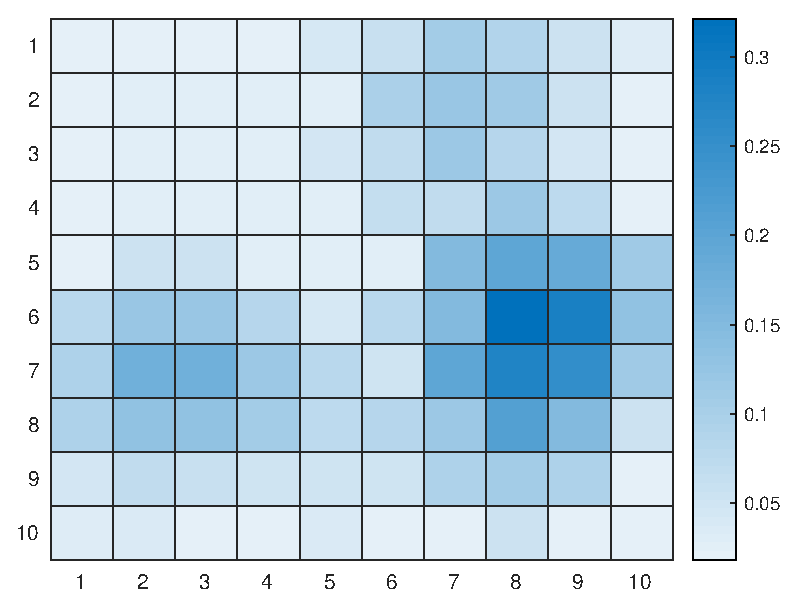
\includegraphics[width=.3\textwidth]{./fig/gridrand10}
}
\subfigure[$\Gamma =40$]{
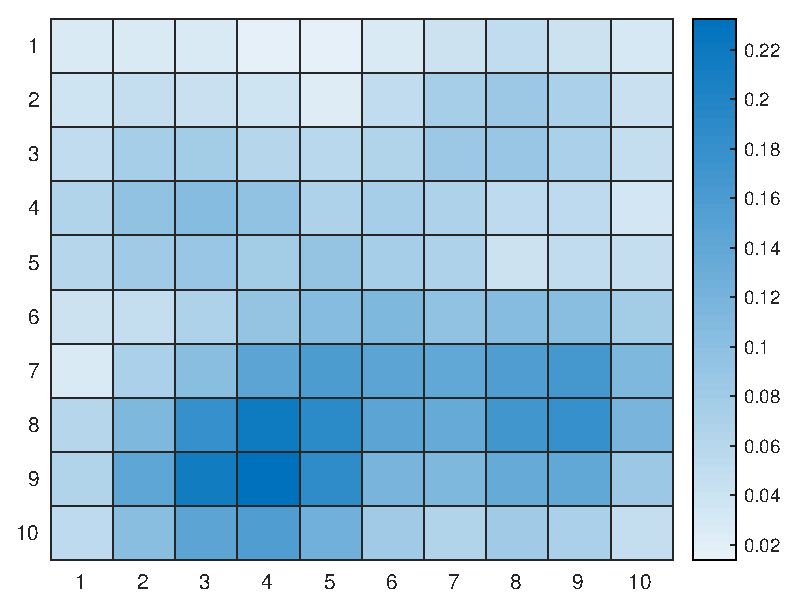
\includegraphics[width=.3\textwidth]{./fig/gridrand40}
}
\subfigure[$\Gamma =60$]{
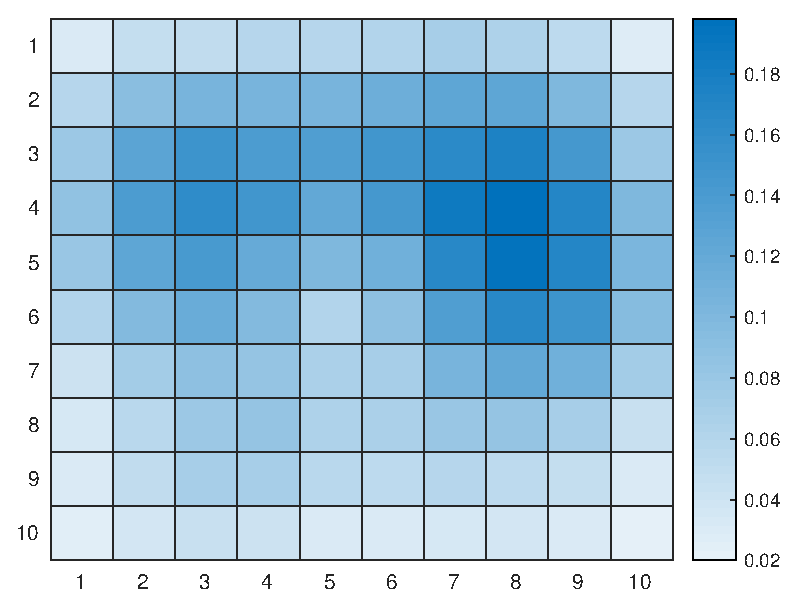
\includegraphics[width=.3\textwidth]{./fig/gridrand60}
}
\subfigure[$\Gamma =80$]{
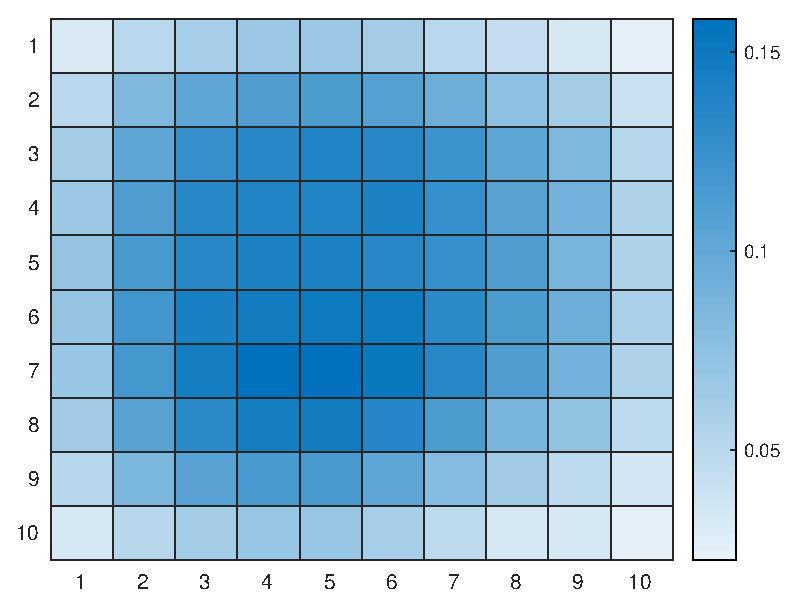
\includegraphics[width=.3\textwidth]{./fig/gridrand80}
}
\subfigure[$\Gamma =90$]{
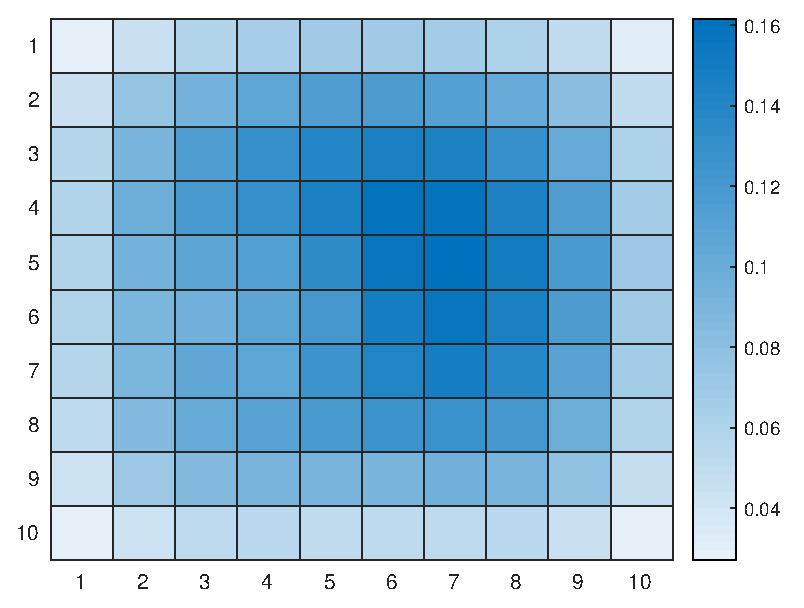
\includegraphics[width=.3\textwidth]{./fig/gridrand90}
}
\subfigure[$\Gamma =95$]{
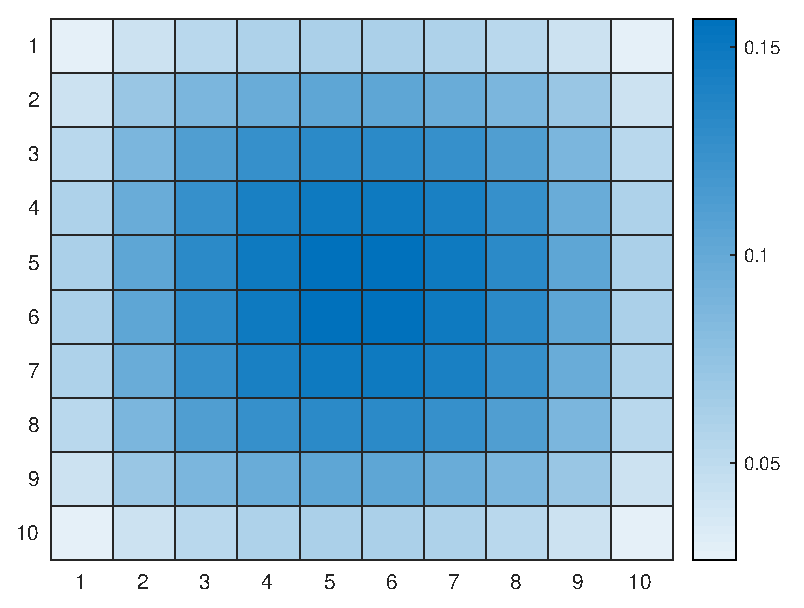
\includegraphics[width=.3\textwidth]{./fig/gridrand95}
}
\subfigure[Katz]{
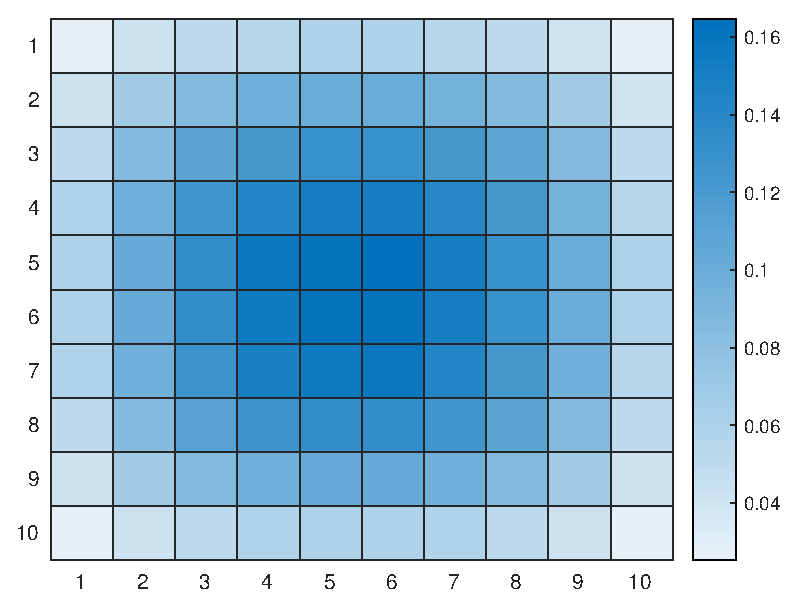
\includegraphics[width=.3\textwidth]{./fig/gridkatz}
}
\caption{Visualization of centrality values of a $10 \times 10$ grid graph. The nodes in $V'$ are chosen at random. Even for a large number of $\Gamma$, we see differences in the central nodes}
\label{fig:grid}
\end{figure}

\begin{figure}[t]
\centering
\subfigure[$\Gamma \approx 5\%$]{
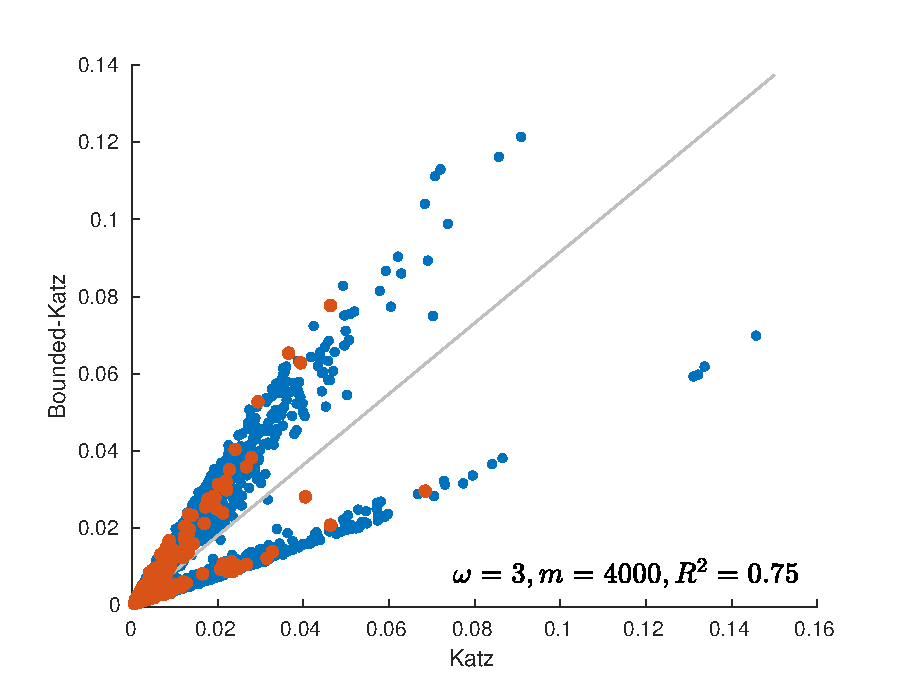
\includegraphics[width=.45\textwidth]{./fig/twitter05}
}
\subfigure[$\Gamma \approx10\%$]{
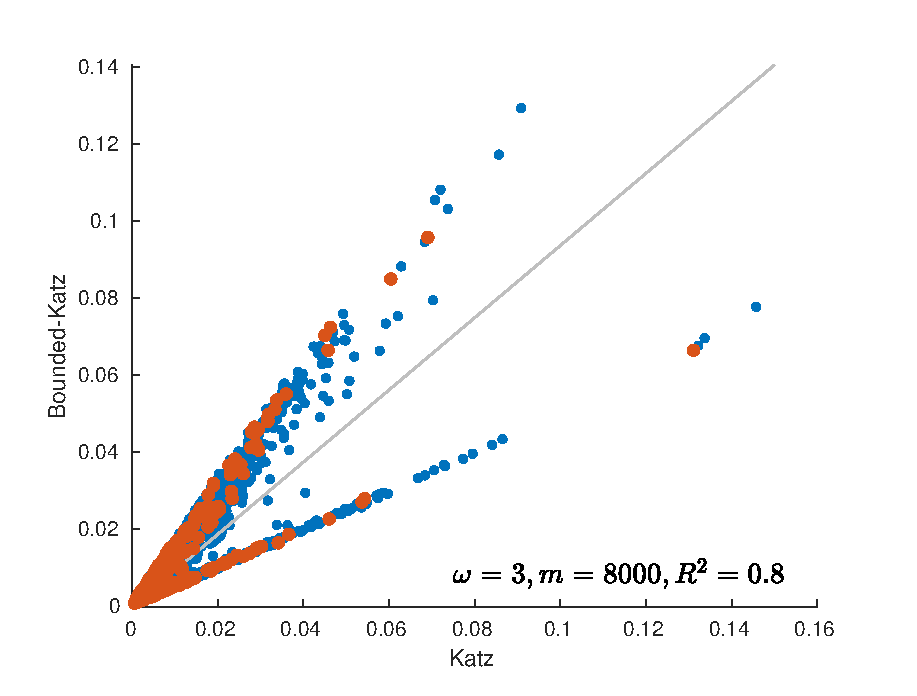
\includegraphics[width=.45\textwidth]{./fig/twitter1}
}
\subfigure[$\Gamma \approx 20\%$]{
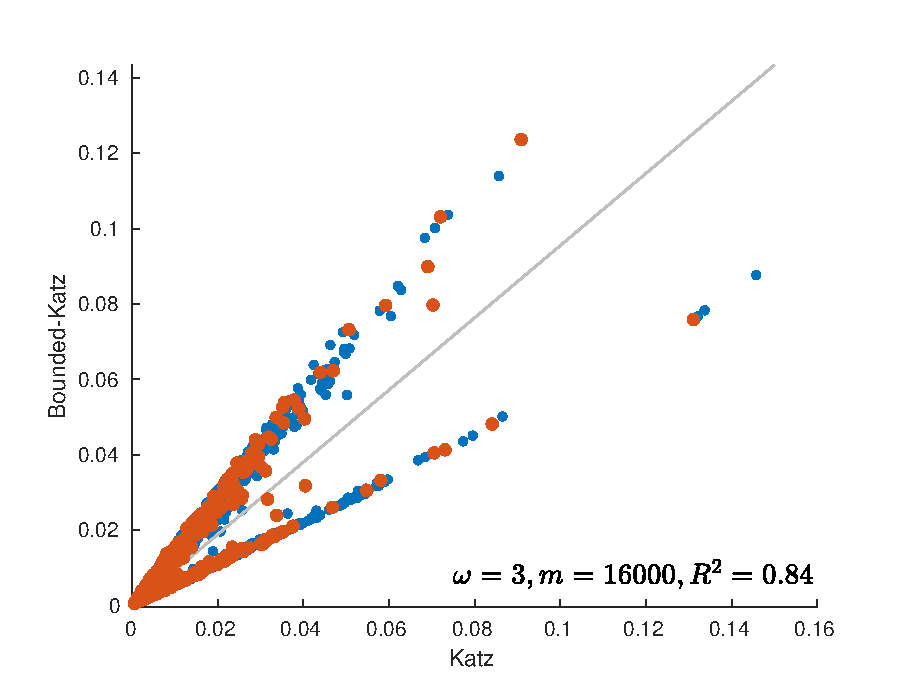
\includegraphics[width=.45\textwidth]{./fig/twitter20}
}
\subfigure[$\Gamma \approx 30$]{
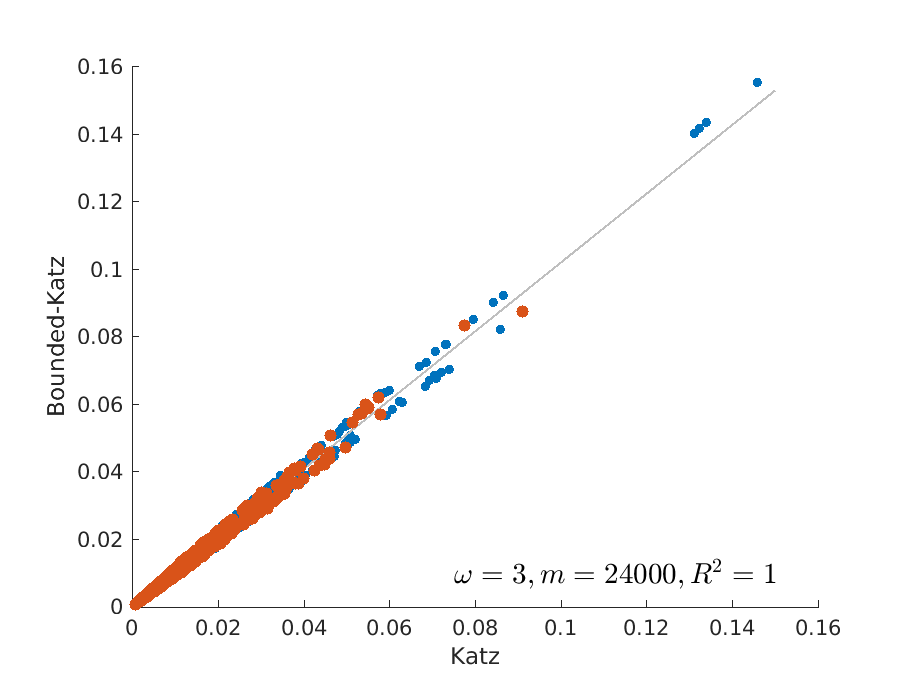
\includegraphics[width=.45\textwidth]{./fig/twitter30}
}

\caption{Twitter data. Directed graph}
\label{fig:twitter}
\end{figure}

\begin{figure}[t]
\centering
\subfigure[$\Gamma \approx 1\%$]{
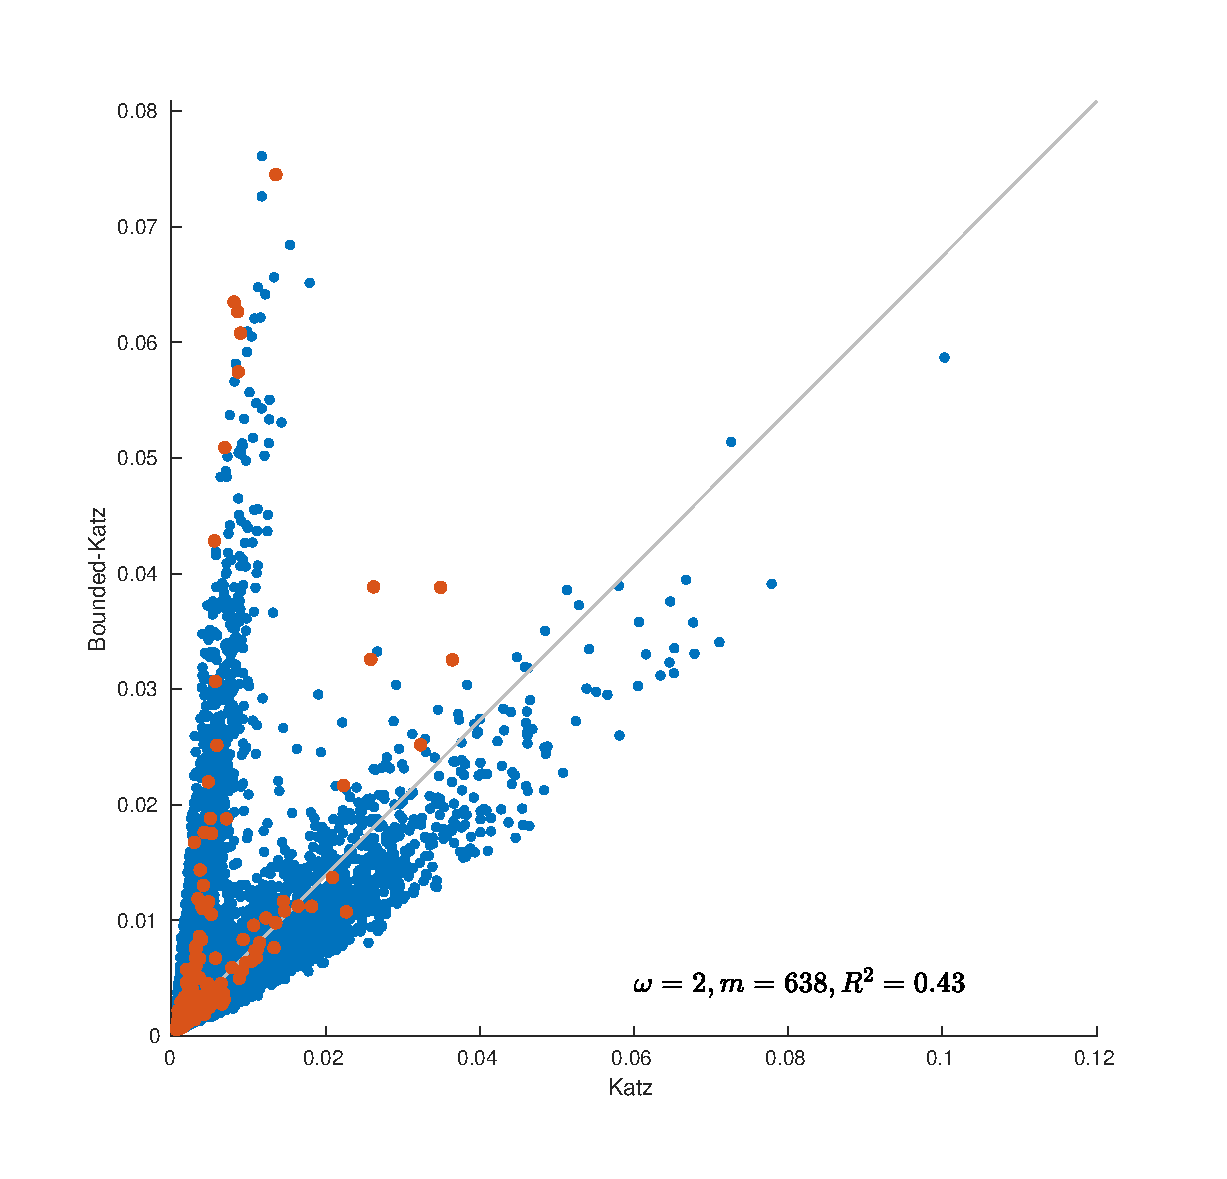
\includegraphics[width=.45\textwidth]{./fig/fb1}
}
\subfigure[$\Gamma \approx 2\%$]{
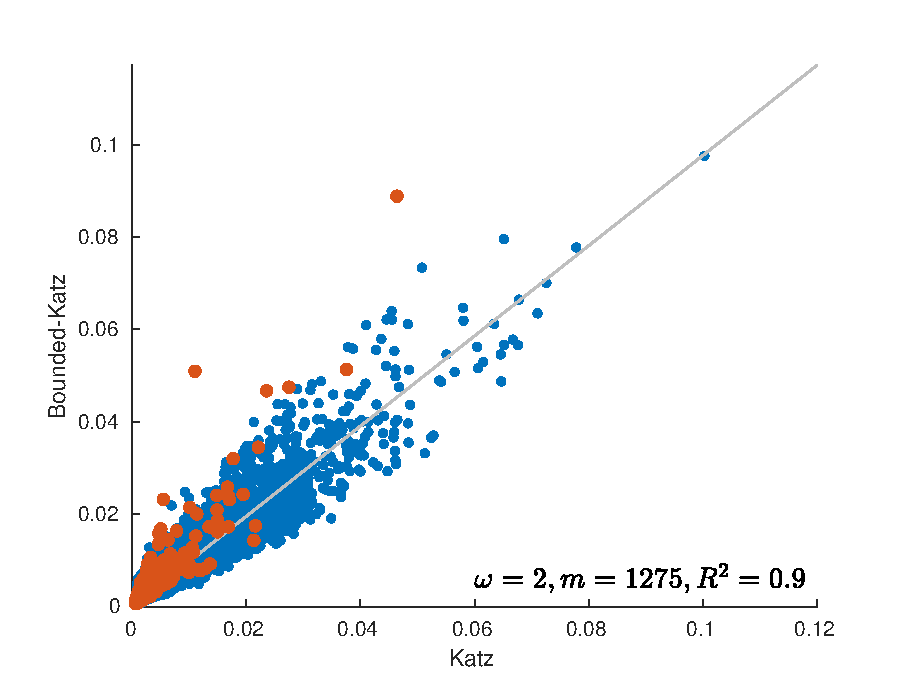
\includegraphics[width=.45\textwidth]{./fig/fb2}
}
\subfigure[$\Gamma \approx 4\%$]{
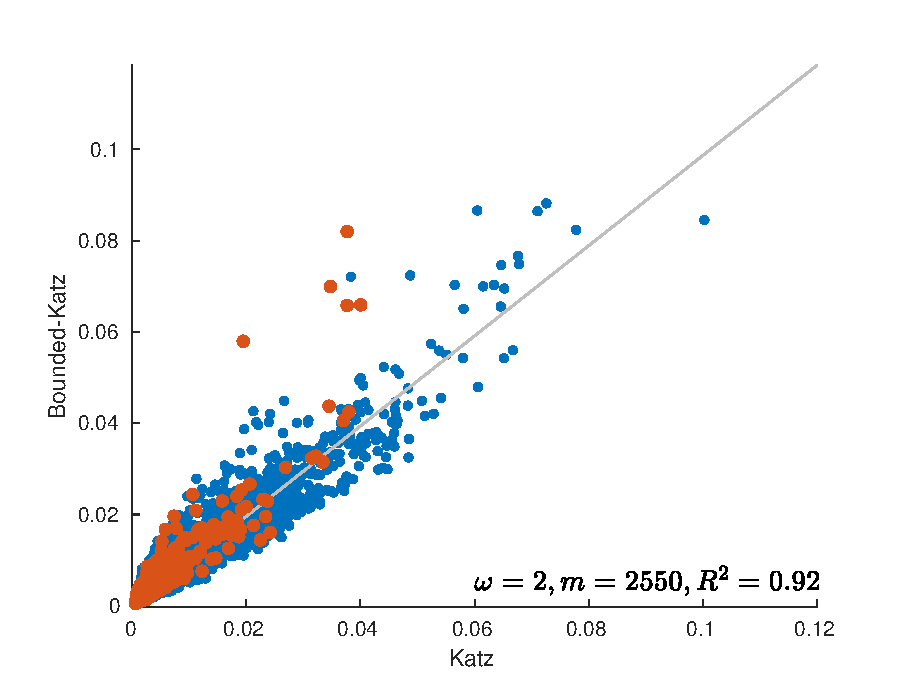
\includegraphics[width=.45\textwidth]{./fig/fb4}
}
\subfigure[$\Gamma \approx 8\%$]{
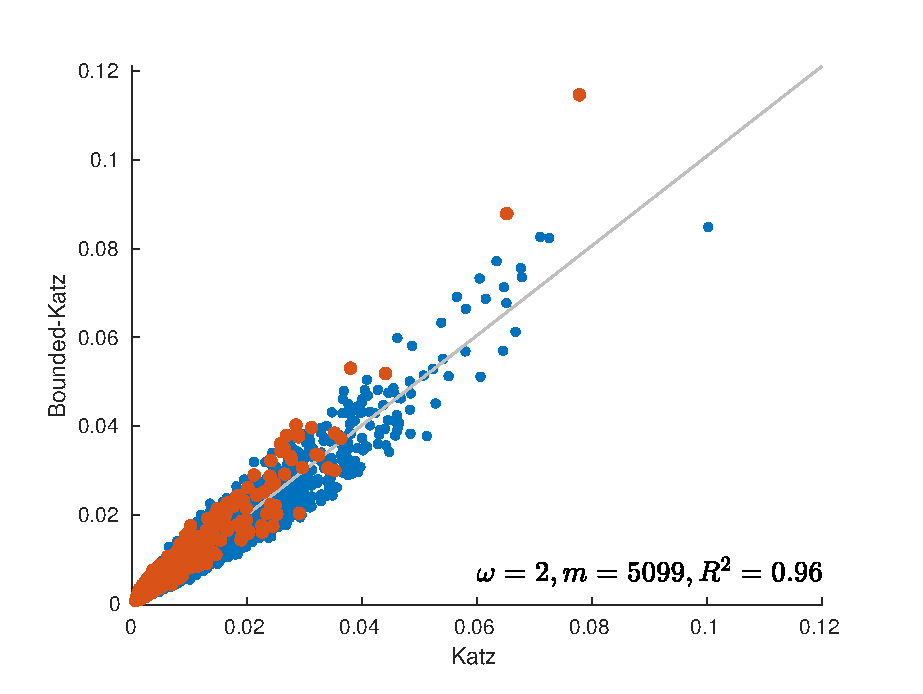
\includegraphics[width=.45\textwidth]{./fig/fb8}
}

\caption{Facebook data. Undirected graph}
\label{fig:fb}
\end{figure}
\subsection{Random Walk Betweenness Centrality}

Consider the betweenness centrality measure based on random walks (RWBC) proposed in \cite{newman2005measure}. Unlike the standard betweenness centrality measure that only only considers shortest paths between a pair of nodes, their measure considered all paths while giving more importance to shorter paths.  They define the betweenness of a vertex $i$ as the ``net'' number of times a walk passes through $i$. By ``net'' the authors meant that if a walk passes through $i$ and later passes back through it in the opposite direction, the two would cancel out and their is no contribution to the betweenness. 

RWBC was was originally proposed for undirected graphs. It can easily be adjusted for directed graphs as follows: Let $A$ adjacency matrix with $D_{out}$ and $D_{in}$ the out and in-degree matrices respectively of a directed graph. Define the transition matrix of this graph as 
\begin{equation}
M = D^{-1}_{out}A
\end{equation}
Note: For vertices with out-degree zero, add a self-loop to them making their out-degree one.

For a walk starting at $s$, the probability that it is at $j$ after $r$ steps is given by $[M^r]_{sj}$. The probability that the walk continues further to an adjacent vertex $i$ is $[M^r]_{sj}k^{-1}_{j}$, where $k^{-1}_{j}$ is the out-degree at $j$. Summing over all possible values of $r$ we get the matrix
\begin{equation}
(I - M)^{-1}D^{-1}_{out} = (D_{out} - A )^{-1}
\end{equation}
Assume $(D_{out} - A )^{-1}$ exists. If not we can remove a row and column. 

Let $\textbf{s}$ be the vector given by 
\begin{equation*}
s_i = \begin{cases}
1,& \text{if } i = s\\
-1,& \text{if } i = t\\
0, &\text{otherwise}
\end{cases}
\end{equation*}
and let $\textbf{V}$ be the vector 
\begin{equation}
\textbf{V} = (D_{out}-A)^{-1}\textbf{s}
\end{equation}


    The net flow of random walk through the $i$th vertex is for a given $s$-$t$ pair is given by
    \begin{equation}
    I_i = \sum_{(i,j)\in E} |V_i - V_j|
    \end{equation}
    \subsection{Flow Based Betweenness Centrality}
%	\section{Medial Measures}
 %   With regard to the current state of the road network (WCL deployment), how important is a given node as a potential installation location?
    


    \subsection{Betweenness Centrality}
    For a given path, $p$, let $r(p)$ be the fraction of $p$ that can be completed with a full charge. The following centrality measure of a node $v \in V$ is proposed
    
    \begin{equation}
    c(v) = \sum_{i=1}^{diam(G)} \alpha_i \sum_{\substack{s, t \in V\\s \neq t}} \frac{\delta_{s,t}^i(v)}{\delta_{s,t}^i}
    \end{equation}
	\subsection{Group Betweenness Centrality}
	
	The \emph{Group Betweenness Centrality} (GBS) \citep{everett1999centrality, dolev2009incremental} for $C \subset V$, is given by:
	\begin{equation*}
		GBC(C) = \sum_{s \neq t \in V}\frac{\sigma_{s,t}(C)}{\sigma_{s,t}}
	\end{equation*}
	where $\sigma_{s,t}(C)$ is the number of $s$-$t$ shortest paths that contain at least one node in $C$. 
	
	The \textbf{Maximum Betweenness Centrality} (MBC) is the problem of finding $|C| =k$, that maximizes the probability of detecting communication between a pair of nodes $s$ and $t$ chosen uniformly at random. It is assumed that the communication is realized along shortest paths which
	are, again, selected uniformly at random. This is equivalent to finding $C \subset V$ such that $GBC(C)$ is maximized for a given budget, $b$ such that $c(C) \leq b$ where $c:V \to \mathbb{R}_{>0}$ is a cost function on the nodes.
	
	With the application of electric-vehicle charging, we introduce \emph{charge-gain betweenness centrality} (CGGBC) given by
	\begin{align*}
		CGGBC(C) &= \sum_{s \neq t \in V}\bar{f}_{s,t}(C) - \epsilon_{s,t}\\
		&=  \sum_{s \neq t \in V}\bar{f}_{s,t}(C) - \sum_{s \neq t \in V} \epsilon_{s,t}\\
		&= \sum_{s \neq t \in V}\frac{F{s,t}(C)}{\sigma_{s,t}} - \sum_{s \neq t \in V} \epsilon_{s,t}\\
	\end{align*}
	where $\bar{f}_{s,t}(C) $ is the average final charge of all $s$-$t$ shortest paths with $C$,\\ $\epsilon_{s,t}$ is the final charge without $C$, and \\
	$F_{s,t}(C)$ is the sum of all final charges with $C$.
	
	\noindent The term $\epsilon_{s,t}$ is a constant and can all together be dropped when finding $C$ that maximizes $CGGBC$. Thus we are interested in:
	\begin{equation}
	\max_{C \subset V, |C| \leq k} \ \ \sum_{s \neq t \in V}\frac{F{s,t}(C)}{\sigma_{s,t}}.
	\end{equation}
	
	\noindent CBBGC is a generalized version of MBC and  \cite{puzis2007finding} showed that MBC is NP-hard.
	\section{Models}
\section{Experiments}
	\subsection{Greedy Algorithm}
	\begin{algorithm}
		\caption{Greedy Algorithm}\label{euclid}
		
		\begin{algorithmic}[1]
			\State \textbf{Input:} $G = (V,E), c, b$
			\State $H := \emptyset$
			\State $\textit{stringlen} \gets \text{length of }\textit{string}$
			\State $i \gets \textit{patlen}$
			\If {$i > \textit{stringlen}$} \Return false
			\EndIf
			\State $j \gets \textit{patlen}$
			\If {$\textit{string}(i) = \textit{path}(j)$}
			\State $j \gets j-1$.
			\State $i \gets i-1$.
			\State \textbf{goto} \emph{loop}.
			\State \textbf{close};
			\EndIf
			\State $i \gets i+\max(\textit{delta}_1(\textit{string}(i)),\textit{delta}_2(j))$.
			\State \textbf{goto} \emph{top}.
		\end{algorithmic}
	\end{algorithm}
    \subsection{Theoretical Results}
	\section{Applications}
    \begin{enumerate}
    \item EV SOC
    \item Water networks, optimal pump schedule 
        \end{enumerate}

    \section{Notes}
    The control of the spectral centrality has been studied from different points of view:
    Topology Control. Lately, the question of how to modify the topology of the network in order to control the centrality
score of nodes became a subject of interest.

In an "collapsing social network" the set $V'$ can be the very active users,, or the dedicated users. The premium plus users. Users who pay a monthly fee.


\cite{pei2015detecting} Plenty of phenomena in various domains can be modelled by the spreading dynamics in social network, e.g, contagious diseases, piece of information, advertisement. The detection of spreading processes in social networks is an is important as it can lead to timely intervention measures during the spread of an epidemic, and surveilance of current trending topics in online social networks. Surveillance in the network can be performed by placing sensors in the network. In \citep{leskovec2007cost}, a heuristic for the optimal placement of sensors is proposed that can detect contagious outbreaks before they happen by taking advantage of the informative properties of the social network.
    
 Facebook data \citep{viswanath-2009-activity}. Charging units are considered to be users in a network with high interest in a particular story who are also wiling to spread information the piece of information. Thus if marketing companies can first identify the "charging nodes". These can be gotten by considering historical data if a user is active in sharing similar information. 
 
 \cite{zhang2013rumor} In an
early psychological experiment, researchers found about 70\% of details in a rumor were lost in the first six mouth-to-mouth transmissions. Rumor spreading is a fundamental topic in psychology and sociology.; Rumor spreading on social networks has recently attracted a lot of scientific research \textbf{[many cite]}. When the average path length of the network is short, rumors can be disseminated globally. In real social networks,  the rumor spreading process in more complex \textbf{[cite, cite]}. The rumor evolves constantly in its spreading process, which grows shorter, more concise, more easily grasped, and told \textbf{[cite]}. The behavior originates from the cummulative modifications during the spreading process, which is sometimes called "chinese whispers" or "Telephone \textbf{[cite]}. For example, in Twitter, once a user discusses a certain topic, his or her followers will understand the topic differently. If it is a rumor, the following discussions can be roughly classified as affirmative, negative, curious, unrelated, and unknown arguments \textbf{[cite]}. No matter what class it belongs to, they are non the less variants of the original rumor. Thus, whether the original rumor can infect the whole network depends not only on the existence of the connections among individuals, but also their strategies. The strategies can are divided into two classes, forward directly or change it before spreading it out. i.e Forwarders and modifiers. In email systems, modifiers can not only be users but also machines, called remailers \textbf{[cite]}. Most work has been on networks of only forwarders.  \cite{zhang2013rumor} takes both forwarders and modifiers into account. \textbf{[cite 3 -8]} takes a spreading rate and an annihilation rate as two key parameters. 
The original rumor model by \citep{daley1964epidemics}, individuals can play three roles, ignorants, spreaders, and stiflers. 
 
 \citep{agliari2006efficiency} The propagation of information can be seen as a sequence of interpersonal processes between the interacting agents in the system. 
 
\citep{wu2004information} the observation that an item
relevant to one person is more likely to be of interest to individuals in the same social circle than those outside of it. An epidemic model on a scale-free network with this property has a finite threshold, implying that the spread of information is limited. Information is selective and passed by its host only to individuals the host thinks would be interested in it. This paper introduces an epidemic model with decay in the transmission probability of a particular piece of information as function of the distance between the originating source and current potential target.  They show that the spread of information on a scale-free network is limited. 

\citep{brashears2016error} Humans make mistake but diffusion through social networks is modeles as though they do not. 

\citep{tutzauer2007entropy} “most of the sociologically interesting processes are not covered by the major measures” of centrality (p. 63).
What properties should a measure of centrality possess if it is to describe nodes in a pathtransfer network?

Example. A puzzle being solved in a network moving from individual to individual. A each step the puzzle gets easier and after k steps the puzzle is solved. e.g a crossword puzzle with $km$ letters to be added. At each step, a person must add $m$ letters before chosing at random who to send it to. Assume they are they are people in the network who reset the puzzle once they recieve it. Most central node is one who gets the puzzle the most times. 

A random web surfer clicks on surfs the web. However, he has patience to only make k visits before he gives up if he doesn't find what he wants. There are however some webpages that are related to what the surfer wants thus if he finds one of these his motivation to randomly surf another $k$ pages is renewed. If this process is to be taken, what are the most important websites that he should start with. What should a google search give him? A ranking on the webpages based on this. 

Pollen travels on bees. Some areas may have many flowers with pollen. A flower is a refueling station

Consider a dooms day scenario, all fuel stations are empty. Where is the best place for an emergence vehicle to start from in order for it to move through the network and help as many locations. Here the motion could be at random. In wide spread emergencies in the city, what are the best place to locate emergency stations. 


\cite{akyildiz2002wireless} Wireless sensor networks are prone to high error rates. 

\citep{wan2002psfq} Most wireless sensor networks consist of very cheap devices that are prone to high error rates. However, for the applications they are designed for, for example temperature monitoring or animal location tracking, they do not require reliable data delivery. Thus occotional loss of sensor reading is tolerable. Directed diffusion \textbf{[cite]} is one of a represenative class of data dissemination mechanisms, specifically designed for a general class of application in sensor networks. Directed diffusion providews robust dissemination through the use of multi-path forwarding, but the correction reception of all data messages is not assured. They observed in the context of sensor networks, data that flows from sources to sinks is generally tolerable to loss. On the other hand, however, data that flows from sinks to sources for the purpose of control or management (e.g, retasking sensors) is sensitive to message loss. For example, disseminating a program image to sensor nodes is problematic. Loss of a single message associated with code segment or script would render the image useless and the re-tasking operation a failure. ... Error accumulates exponentially ovr multihops. To simply illustrate this, assume that a packet error rate of a wireless channel is $p$, then the chances of exchanging a message sucessfully across a single hop is $(1-p)$. The probablity that a message is successfully recieved across $n$ hops is $(1-p)^n$. \textbf{Note:} In our centrality work, a define their succession rate probability $p_k$ and $k$, the number of steps parameter can be chosen such that $p_k > (1-p)^k$ 

\citep{nakamura2007information} A Wireless Sensor Network (WSN) [Pottie and Kaiser 2000; Akyildiz et al. 2002] is aspecial type of ad hoc network composed of a large number of nodes equipped with different sensor devices. This network is supported by technological advances in lowpowerm wireless communications along with silicon integration of various functionalities
such as sensing, communication, and processing. WSNs are emerging as an important
computer class based on a new computing platform and networking structure that will
enable novel applications that are related to different areas such as environmental
monitoring, industrial and manufacturing automation, health-care, and military. Commonly,
wireless sensor networks have strong constraints regarding power resources
and computational capacity

\cite{cuzzocrea2012edge} Centrality for wireless sensor networks for topology-control
protocol for sensor networks.

\cite{tian2005randomwalk} Routing in WSN based on random walks
% --------------------------------------------------------------

%     You don't have to mess with anything below this line.
	% --------------------------------------------------------------
	\bibliographystyle{plain}
	\bibliography{bib}
\end{document}


